\chapter{Diseño e implementación} % Main chapter title
\label{Chapter3} 

En este capítulo se explica como se utilizaron las herramientas mencionadas en el capítulo 2 para resolver los objetivos del trabajo presentados en el capítulo 1.

% Change X to a consecutive number; for referencing this chapter elsewhere, use \ref{ChapterX}

\definecolor{mygreen}{rgb}{0,0.6,0}
\definecolor{mygray}{rgb}{0.5,0.5,0.5}
\definecolor{mymauve}{rgb}{0.58,0,0.82}

%%%%%%%%%%%%%%%%%%%%%%%%%%%%%%%%%%%%%%%%%%%%%%%%%%%%%%%%%%%%%%%%%%%%%%%%%%%%%
% parámetros para configurar el formato del código en los entornos lstlisting
%%%%%%%%%%%%%%%%%%%%%%%%%%%%%%%%%%%%%%%%%%%%%%%%%%%%%%%%%%%%%%%%%%%%%%%%%%%%%
\lstset{ %
  backgroundcolor=\color{white},   % choose the background color; you must add \usepackage{color} or \usepackage{xcolor}
  basicstyle=\footnotesize,        % the size of the fonts that are used for the code
  breakatwhitespace=false,         % sets if automatic breaks should only happen at whitespace
  breaklines=true,                 % sets automatic line breaking
  captionpos=b,                    % sets the caption-position to bottom
  commentstyle=\color{mygreen},    % comment style
  deletekeywords={...},            % if you want to delete keywords from the given language
  %escapeinside={\%*}{*)},          % if you want to add LaTeX within your code
  %extendedchars=true,              % lets you use non-ASCII characters; for 8-bits encodings only, does not work with UTF-8
  %frame=single,	                % adds a frame around the code
  keepspaces=true,                 % keeps spaces in text, useful for keeping indentation of code (possibly needs columns=flexible)
  keywordstyle=\color{blue},       % keyword style
  language=[ANSI]C,                % the language of the code
  %otherkeywords={*,...},           % if you want to add more keywords to the set
  numbers=left,                    % where to put the line-numbers; possible values are (none, left, right)
  numbersep=5pt,                   % how far the line-numbers are from the code
  numberstyle=\tiny\color{mygray}, % the style that is used for the line-numbers
  rulecolor=\color{black},         % if not set, the frame-color may be changed on line-breaks within not-black text (e.g. comments (green here))
  showspaces=false,                % show spaces everywhere adding particular underscores; it overrides 'showstringspaces'
  showstringspaces=false,          % underline spaces within strings only
  showtabs=false,                  % show tabs within strings adding particular underscores
  stepnumber=1,                    % the step between two line-numbers. If it's 1, each line will be numbered
  stringstyle=\color{mymauve},     % string literal style
  tabsize=2,	                   % sets default tabsize to 2 spaces
  title=\lstname,                  % show the filename of files included with \lstinputlisting; also try caption instead of title
  morecomment=[s]{/*}{*/}
}


%----------------------------------------------------------------------------------------
%	SECTION 1
%----------------------------------------------------------------------------------------
\section{Generación del entorno base para el desarrollo del sistema de backend}
 
%La idea de esta sección es resaltar los problemas encontrados, los criterios utilizados y la justificación de las decisiones que se hayan tomado.

%Se puede agregar código o pseudocódigo dentro de un entorno lstlisting con el siguiente código:

%\begin{verbatim}
%\begin{lstlisting}[caption= "un epígrafe descriptivo"]
%	las líneas de código irían aquí...
%\end{lstlisting}
%\end{verbatim}

%A modo de ejemplo:

%\begin{lstlisting}[label=cod:vControl,caption=Pseudocódigo del lazo principal de control.]  % Start your code-block

%#define MAX_SENSOR_NUMBER 3
%#define MAX_ALARM_NUMBER  6
%#define MAX_ACTUATOR_NUMBER 6

%uint32_t sensorValue[MAX_SENSOR_NUMBER];		
%FunctionalState alarmControl[MAX_ALARM_NUMBER];	//ENABLE or DISABLE
%state_t alarmState[MAX_ALARM_NUMBER];						//ON or OFF
%state_t actuatorState[MAX_ACTUATOR_NUMBER];			//ON or OFF

%void vControl() {

%	initGlobalVariables();
	
%	period = 500 ms;
		
%	while(1) {

%		ticks = xTaskGetTickCount();
		
%		updateSensors();
		
%		updateAlarms();
		
%		controlActuators();
		
%		vTaskDelayUntil(&ticks, period);
%	}
%}
%\end{lstlisting}
\section{Broker Mosquitto}

El broker Mosquitto es una parte central del sistema ya que se encarga de distribuir los mensajes entre los distintos elementos del sistema. El único requisito es que se encuentre instalado en la misma red que los clientes (en un sistema que no requiere de muchos recursos). Su instalación, en un entorno operativo Ubuntu se realiza con los siguientes comandos:




\begin{lstlisting}[caption=  Instalación/lanzamiento del broker Mosquitto]
		sudo apt-get install mosquitto mosquitto-clients
		sudo systemctl enable mosquitto.service
\end{lstlisting}

Para configurarlo se debe editar el archivo : "/etc/mosquitto/mosquitto.conf":

\begin{lstlisting}[caption=  Contenido archivo mosquitto.conf]
log_dest file /var/log/mosquitto/mosquitto.log

include_dir /etc/mosquitto/conf.d
listener 9001
protocol websockets
allow_anonymous true

\end{lstlisting}

En este archivo, se especifíca los puertos que se utilizará, en este caso, el puerto 9001 con el protocolo Websockets. Se permite la interconexión de cualquier cliente y el archivo donde se guardará un log de todos los eventos se encuentra en la ubicación "/var/log/mosquitto/mosquitto.log".

\pagebreak
\section{Sistema Docker}

El archivo docker-compose.yml contiene los siguientes servicios instalados:

\begin{itemize}
\item servidor mysql:




\end{itemize}




\section{Base de datos del sistema}
En esta sección se describiran las distintas tablas que se almacenan en la base de datos y son útiles para el sistema.

\begin{enumerate}

\item Tabla usuarios (\textit{User}): tabla que contiene la información de los usuarios del sistema. El campo id se incrementa automáticamente, es decir, al incorporar un nuevo usuario al sistema la base de datos asigna el id (se utiliza este campo como llave primaria).En el campo contraseña se almacena el hash de la misma(generado con Bcrypt \citep{WEBSITE:31}). En el campo ocupación se almacena uno de valores: "Enfermero","Médico" o "Administrador". El campo estado (\textit{State}) se utiliza en versiones posteriores del sistema.

\begin{figure}[ht]
	\centering
	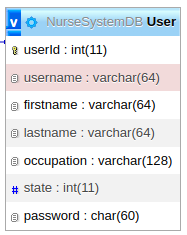
\includegraphics[scale=.7]{./Figures/dB(user).png}
	\caption{Tabla Usuarios.}
	\label{fig:Tabla Usuarios (base de datos)}
\end{figure}

\item Tabla Camas(\textit{Bed}): tabla que contiene la información de las camas como ser su identificación (como en el item anterior se incrementa automáticamente y es clave primaria), ubicación(piso y cuarto) y el número de dispositivo llamador. 

\begin{figure}[ht]
	\centering
	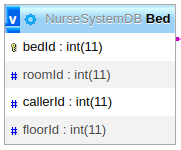
\includegraphics[scale=.7]{./Figures/dB(bed).png}
	\caption{Tabla Camas.}
	\label{fig:Tabla Camas (base de datos)}
\end{figure}

\item Tabla Paciente (\textit{Patient}): tabla que contiene la información de los pacientes. En esta tabla el id no se incrementa automáticamente (ya que puede ser asignado manualmente por el administrador). Ademas, los campos \textbf{bedId}, \textbf{notesTableId} y \textbf{userTableId} contienen claves foraneas que identifican un elemento de la tabla \textit{Bed} (cama), \textit{notesTable} (tablas de notas) y \textit{userTable} (tablas de médicos relacionados al paciente).


\begin{figure}[ht]
	\centering
	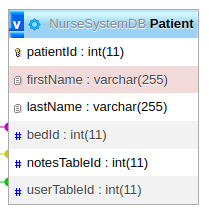
\includegraphics[scale=.7]{./Figures/dB(patient).png}
	\caption{Tabla pacientes.}
	\label{fig:Tabla pacientes (base de datos)}
\end{figure}


\item Relación médicos-pacientes : para generar la relación se utilizan un par de tablas intermedias que permiten que un mismo paciente posea varios médicos tratándolo. Además, un paciente puede utilizar a los mísmos médicos de otro paciente... es una de las ventajas de las bases de datos relacionales.


\begin{figure}[ht]
	\centering
	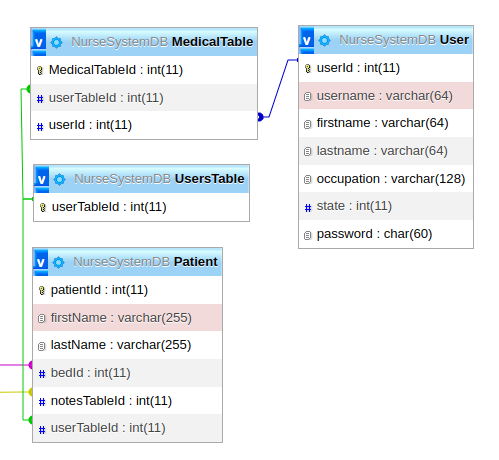
\includegraphics[scale=.45]{./Figures/tabla-medicos-pacientes.png}
	\caption{Relación médicos-pacientes.}
	\label{fig:Relación médicos-pacientes (base de datos)}
\end{figure}



\item Relación tabla de notas- pacientes: como en el caso anterior, se utiliza una tabla de notas generales con una tabla intermedia que los indexa. En este caso y como es particular de cada paciente no se puede repetir.


\begin{figure}[ht]
	\centering
	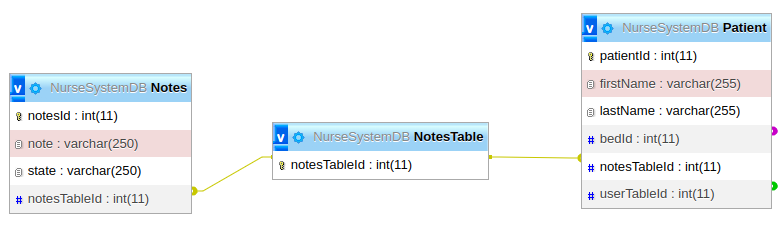
\includegraphics[scale=.45]{./Figures/patient-notes.png}
	\caption{Relación notas-pacientes.}
	\label{fig:Relación notas-pacientes (base de datos)}
\end{figure}

\pagebreak

\item Tabla de eventos programados: En esta tabla se cargan las tareas programadas para un paciente. El identificador se incrementa al generarse, el nro de paciente es enviado por el cliente, el campo tipo de evento puede ser \textbf{diario},\textbf{mensual} o \textbf{diario} y el campo datetime a la hora que se requiere que se realice. El campo nota es donde se coloca la tarea a realizar (Por ejemplo, suministrar X gramos de medicamento Y).


\begin{figure}[ht]
	\centering
	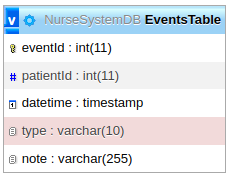
\includegraphics[scale=.45]{./Figures/Events.png}
	\caption{Tabla de eventos programados.}
	\label{fig:Tabla de eventos programados (base de datos)}
\end{figure}


\item Tabla de log eventos: En esta tabla se guardan los eventos relacionados con un paciente. El id se asigna al guardarse el evento. El tipo puede ser \textbf{tarea programada} o \textbf{llamada paciente}. El id del paciente, el id de usuario y la nota se cargan por el usuario que finalizó la accion.


\begin{figure}[ht]
	\centering
	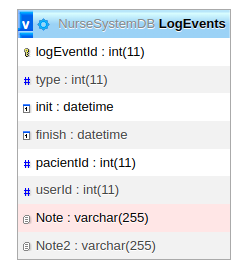
\includegraphics[scale=.45]{./Figures/logEvents.png}
	\caption{Tabla de registro de eventos.}
	\label{fig:Tabla de registro de eventos (base de datos)}
\end{figure}

\item Tabla de especialidades (\textit{SpecTable}): En esta tabla se las distintas especialidades que poseen todos los enfermeros. 

\item Tabla de especialidades de enfermeros (\textit{NurseSpecTable}): En esta tabla se relacionan a los enfermeros con su Id y las distintas especialidades que pueden realizar. Un enfermero puede poseer más de una especialidad.

\item Tabla de tratamientos de pacientes(\textit{PatientSpecTable}): En esta tabla se relacionan a los pacientes con su Id y una tratamiento(se obtiene de la SpecTable). 

\item Tabla de códigos QR (\textit{QRbed}): En esta tabla se almacenan en string los códigos QR correspondientes a las camas para su reconocimiento.

\item Tabla de prioridades (\textit{PriorityTable}): En esta tabla el administrador puede asignar prioridades a las distintas camas del sistema, las prioridades son de 5 niveles, siendo 5 la más alta prioridad.











\end{enumerate}



\section{Sistema de gestión}
\subsection{Descripción de API REST para aplicación Web}
\subsection{Descripción de API MQTT para la mensajeria de la aplicación móvil}


\section{Página Web(frontend)}
\subsection{Estructura y organización del software}
\subsection{Acceso de usuario}
\subsection{Monitoreo del sistema}
\subsection{Gestión de tareas programadas}
\subsection{Estadísticas del sistema}
\section{Aplicación Móvil}
\subsection{Estructura y organización del software}
\subsection{Configuración del broker y acceso de usuario}
\subsection{Modo administrador}
\subsection{Modo médico}
\subsection{Modo enfermera}
\subsection{Interacción médico-enfermera}
\section{Contraste con los requerimientos}
